\documentclass[11pt]{article}

% Insert style guide
\usepackage{my_thesis}

\newcommand\figurescale{1} % set default scaling to 1
% Specifiy the location of images to be used
\graphicspath{{figures/}}

%
\begin{document}
\title{\textsc{Nanoscopy using a semiconductor heterostructure as the sample stage}}
% \date{\footnote{Last Modified: \currenttime, \today.}}

% Create title page
\maketitle


\section{Abstract}
%
% Rewrite abstract mostly from the Xiaodong's feedback
A special structured illumination microscopy scheme using a two dimensional electron gas as the sample stage is proposed. Terahertz plasma waves generated by a current driven instability illuminate the sample. Meanwhile, a plane wave is used to shift the plasmonic pattern needed to expand the observable range of spatial frequencies. Full coverage of the spatial frequency regime is obtained by tuning the plasma waves through gate voltage control. Hence, it is possible to reconstruct an image with resolution up to two orders of magnitude beyond the diffraction limit. Due to linear nature of the technique, only a weak illumination signal is required, therefore minimizing the chances of radiation damage to the  sample.
%
\section{Introduction}
%
% As suggested by Xiaodong, discussion on confocal microscopy is unnecessarily long, and bloating this section. Trim it!
In conventional wide-field fluorescent microscopy, a sample is uniformly illuminated by a beam of light, and the resulting fluorescence is observed in the far-field through the objective lens. The uniform intensity of the illumination along the sample fundamentally restricts the resolution of the system to half the wavelength of light due to the Abbe diffraction limit. With ever growing need to image tiny objects especially in life sciences, modern microscopy techniques such as confocal and linear structured illumination microscopy (SIM) use spatially non-uniform sources of light to illuminate the sample, resulting in resolution extending beyond the diffraction limit by a factor of $2$ \cite{Minsky1988,Gustafsson2000}. Use of pinholes in confocal microscopy makes the technique highly inefficient as a significant portion of light is discarded and it may leave weakly fluorescent objects undetectable. Structured Illumination microscopy is a wide-field technique in which a fine illumination pattern such as a sinusoidal standing wave is used to generate \emph{Moiré fringes} in the observed image. The high frequency content is mathematically reconstructed from a series of images acquired by shifting the pattern. Using a non-linear version of SIM, theoretically unlimited resolution can be achieved \cite{Gustafsson_2005}. However, high levels of illumination intensity are required, subjecting the sample to significant radiation damage.

Surface waves are electromagnetic waves existing at the boundary of a medium having wavelength and phase velocity much smaller than the homogeneous waves of the same frequency in that given medium. Illuminating a sample by surface waves was first proposed by Nassenstein to realize super-resolution since the sub-diffracted waves contain spatial frequency information of the sample beyond the diffraction limit \cite{Nassenstein1970}. Recently, a plasmonic structured illumination microscopy (PSIM) technique was proposed in which surface plasmons existing at a metal-dielectric interface in which a sample was excited by  optical frequency plane waves \cite{Wei2010}. In another scheme, resolution of up to two orders of magnitude beyond the diffraction limit was achieved through mid-infrared graphene plasmons \cite{Zeng2014}.

In solid-state devices like the  high electron mobility transistor (HEMT), a two-dimensional electron gas (2DEG) formed at the interface of two epitaxially grown semiconductors, acts as a transistor channel where free electron concentration of metal-like proportions is observed without any doping, along with remarkably high electron mobility. Plasma waves originating in the few atoms thick electron channel of field-effect transistors, discovered more than 40 years ago have lately received interest because of the potential to realize terahertz frequency sources and sensors \cite{Dyakonov1993,Dyakonov1996,Popov2005,Otsuji2006,Muravjov2010}. For micro-scale lengths, the channel becomes a plasma cavity where the resonant frequency lies in the far-infrared (terahertz) frequency region and remarkably, can be tuned by varying the gate voltage.


In this work, a nanoscale imaging technique is presented in which subwavelength plasma waves, generated in a transistor channel that can be tuned by controlling gate voltage are used as the illumination pattern required for (SIM). The configuration effectively creates a much larger observable spatial frequency region as compared to a far-infrared (terahertz) plane wave. Due to the linear nature of the scheme, resolution of up to two orders of magnitude beyond the diffraction limit can be obtained with a weak field intensity.
%
\begin{figure}[t!]
  \centering
  \def\svgwidth{\linewidth}
  \input{figures/mstruc_gated.pdf_tex}
  \caption{Sample placed on top of HEMT with back gate and excited by 2D plasmons generated by a direct current}
  \label{fig:struct}
\end{figure}
%
%%%%%%%%%%%%%%%
%%%%%%%%%%%%%%%
%%%%%%%%%%%%%%%
%%%%%%%%%%%%%%%
%%%%%%%%%%%%%%%
%%%%%%%%%%%%%%%
%%%%%%%%%%%%%%%
%%%%%%%%%%%%%%%
%%%%%%%%%%%%%%%
\section{Theory}
\subsection{Dispersion relation}
%
A schematic diagram of the proposed system which is similar to a transistor, is shown in Fig. \ref{fig:struct} where a 2DEG that acts as a transistor channel, is formed at the interface of two semiconductor materials of slightly different band-gap energies. Plasma waves are generated in the channel when the source and drain terminals are driven by a current source. Due to reflections from the conducting boundaries, the channel region forms a cavity in which the plasma waves form a standing wave. The structure is backed by a gate terminal that spans the length $L$ of the channel and spaced a distance $d$ below the 2DEG. The gate capacitively couples with the 2DEG and by varying the voltage, the velocity as well as concentration of electrons in the channel can be controlled. A barrier layer of thickness $h$ separates the sample from the 2DEG.

The dispersion relation that shows a frequency dependent resonance response of plasma waves in the 2D channel is obtained by imposing the transverse resonance condition realized by an equivalent transmission line (TL) circuit \cite{Kastner_1988,Michalski2005}. The 2DEG is modeled as a shunt admittance related to Drude-type surface conductivity,
%
\begin{equation}
  Y_{\sigma} = \sigma_s = \frac{N_s e^2 \tau}{m^{\ast}}\frac{1}{1 + \j \O \tau}
  \label{eq:Y2deg}
\end{equation}
%
where $N_s$ is the surface electron density in the channel, $e$ is the electron charge, $m^{\ast}$ is the effective electron mass in the heterostructure, $\tau$ is the scattering time of electrons, $\O$ is the angular frequency. The dispersion relation is then written as:
%
\begin{equation}
  Y^{\uparrow}(z_0) + Y^{\downarrow}(z_0) + Y_{\sigma} = 0.
  \label{eq:dispersion}
\end{equation}
%
Here $Y^{\uparrow}(z_0)$ and $Y^{\downarrow}(z_0)$ are the upward- and downward-looking TL admittances at $z = 0$,
%
\begin{equation}
  Y^{\uparrow}(z_0) = Y_2 \frac{1 - \Gamma^{\uparrow}(z_0)}{1 + \Gamma^{\uparrow}(z_0)}
  \label{eq:Yup}
\end{equation}
%
\begin{equation}
  Y^{\downarrow}(z_0) = -\j Y_1 \cot (k_{z1} d_1)
  \label{eq:Ydown}
\end{equation}
%
Here, $d_{1,2}$ are the thickness of the first and second layers,
respectively,  $Y_{i}$ and $k_{zi}$ where $i = 0,1,2$ are the respective TM mode admittances and wavenumbers of the corresponding layer given by:
%
\begin{align}
  & Y_i = \frac{\O \E_i \E_0}{k_{zi}}&&k_{zi} = \pm \sqrt{k_0^2 \E_i - k_x^2} \\
  \label{eq:Yandk}
\end{align}
%
where $\E_i$ is the relative permittivity of $i^{\text{th}}$ layer and $k_x$ is the longitudinal propagation constant of the structure. The upward-looking reflection coefficient $\Gamma^{\uparrow}$ in \eqref{eq:Yup} is expressed in terms of the TM mode admittances:
%
\begin{equation}
  \Gamma^{\uparrow}(z_0) = \frac{Y_1 - Y_0}{Y_0 + Y_1} \e^{-2\j k_{z2}d_1}
  \label{eq:Gamma}
\end{equation}
%
% Structure details of GaN/ AlGaN
An analytical solution of \eqref{eq:dispersion} in terms of longitudinal propagation constant $k_x$ is tedious, therefore numerical root-finding techniques such as the Newton method were employed \cite{9780521880688}. As an example, the dispersion relation of a Gallium Nitride / Aluminum Gallium Arsenide (GaN/AlGaN) heterostructure is shown in Fig. \ref{fig:dispersion}. At $25~ \mathrm{THz}$, the plasma propagation constant is 80 times greater than the free-space wavenumber. Such extreme subwavelength phenomenon makes super-resolution possible, extending resolution by two orders of magnitude beyond the diffraction limit. The structure parameters used to compute the dispersion relation via \eqref{eq:Y2deg}-\eqref{eq:Gamma} are now briefly discussed. The gate-channel separation is $d = 100~\mathrm{nm}$. The channel length $L$ is $2~\mathrm{\u m}$ whereas the AlGaN barrier layer is
$h = 20~ \mathrm{nm}$ wide. The permittivity of both semiconductor layers is approximated to the static value, i.e., $\E_1 \approx \E_2 = 9.5$ \cite{Muravjov2010}. A surface carrier density of $N_s = 7.5 \times 10^{12}~ \mathrm{cm}^{-2}$ and scattering time $\tau$ of $114 \mathrm{ps}$ corresponding to a temperature of $3 \mathrm{K}$ is assumed.
%
\begin{figure}[t!]
  \subfloat[]{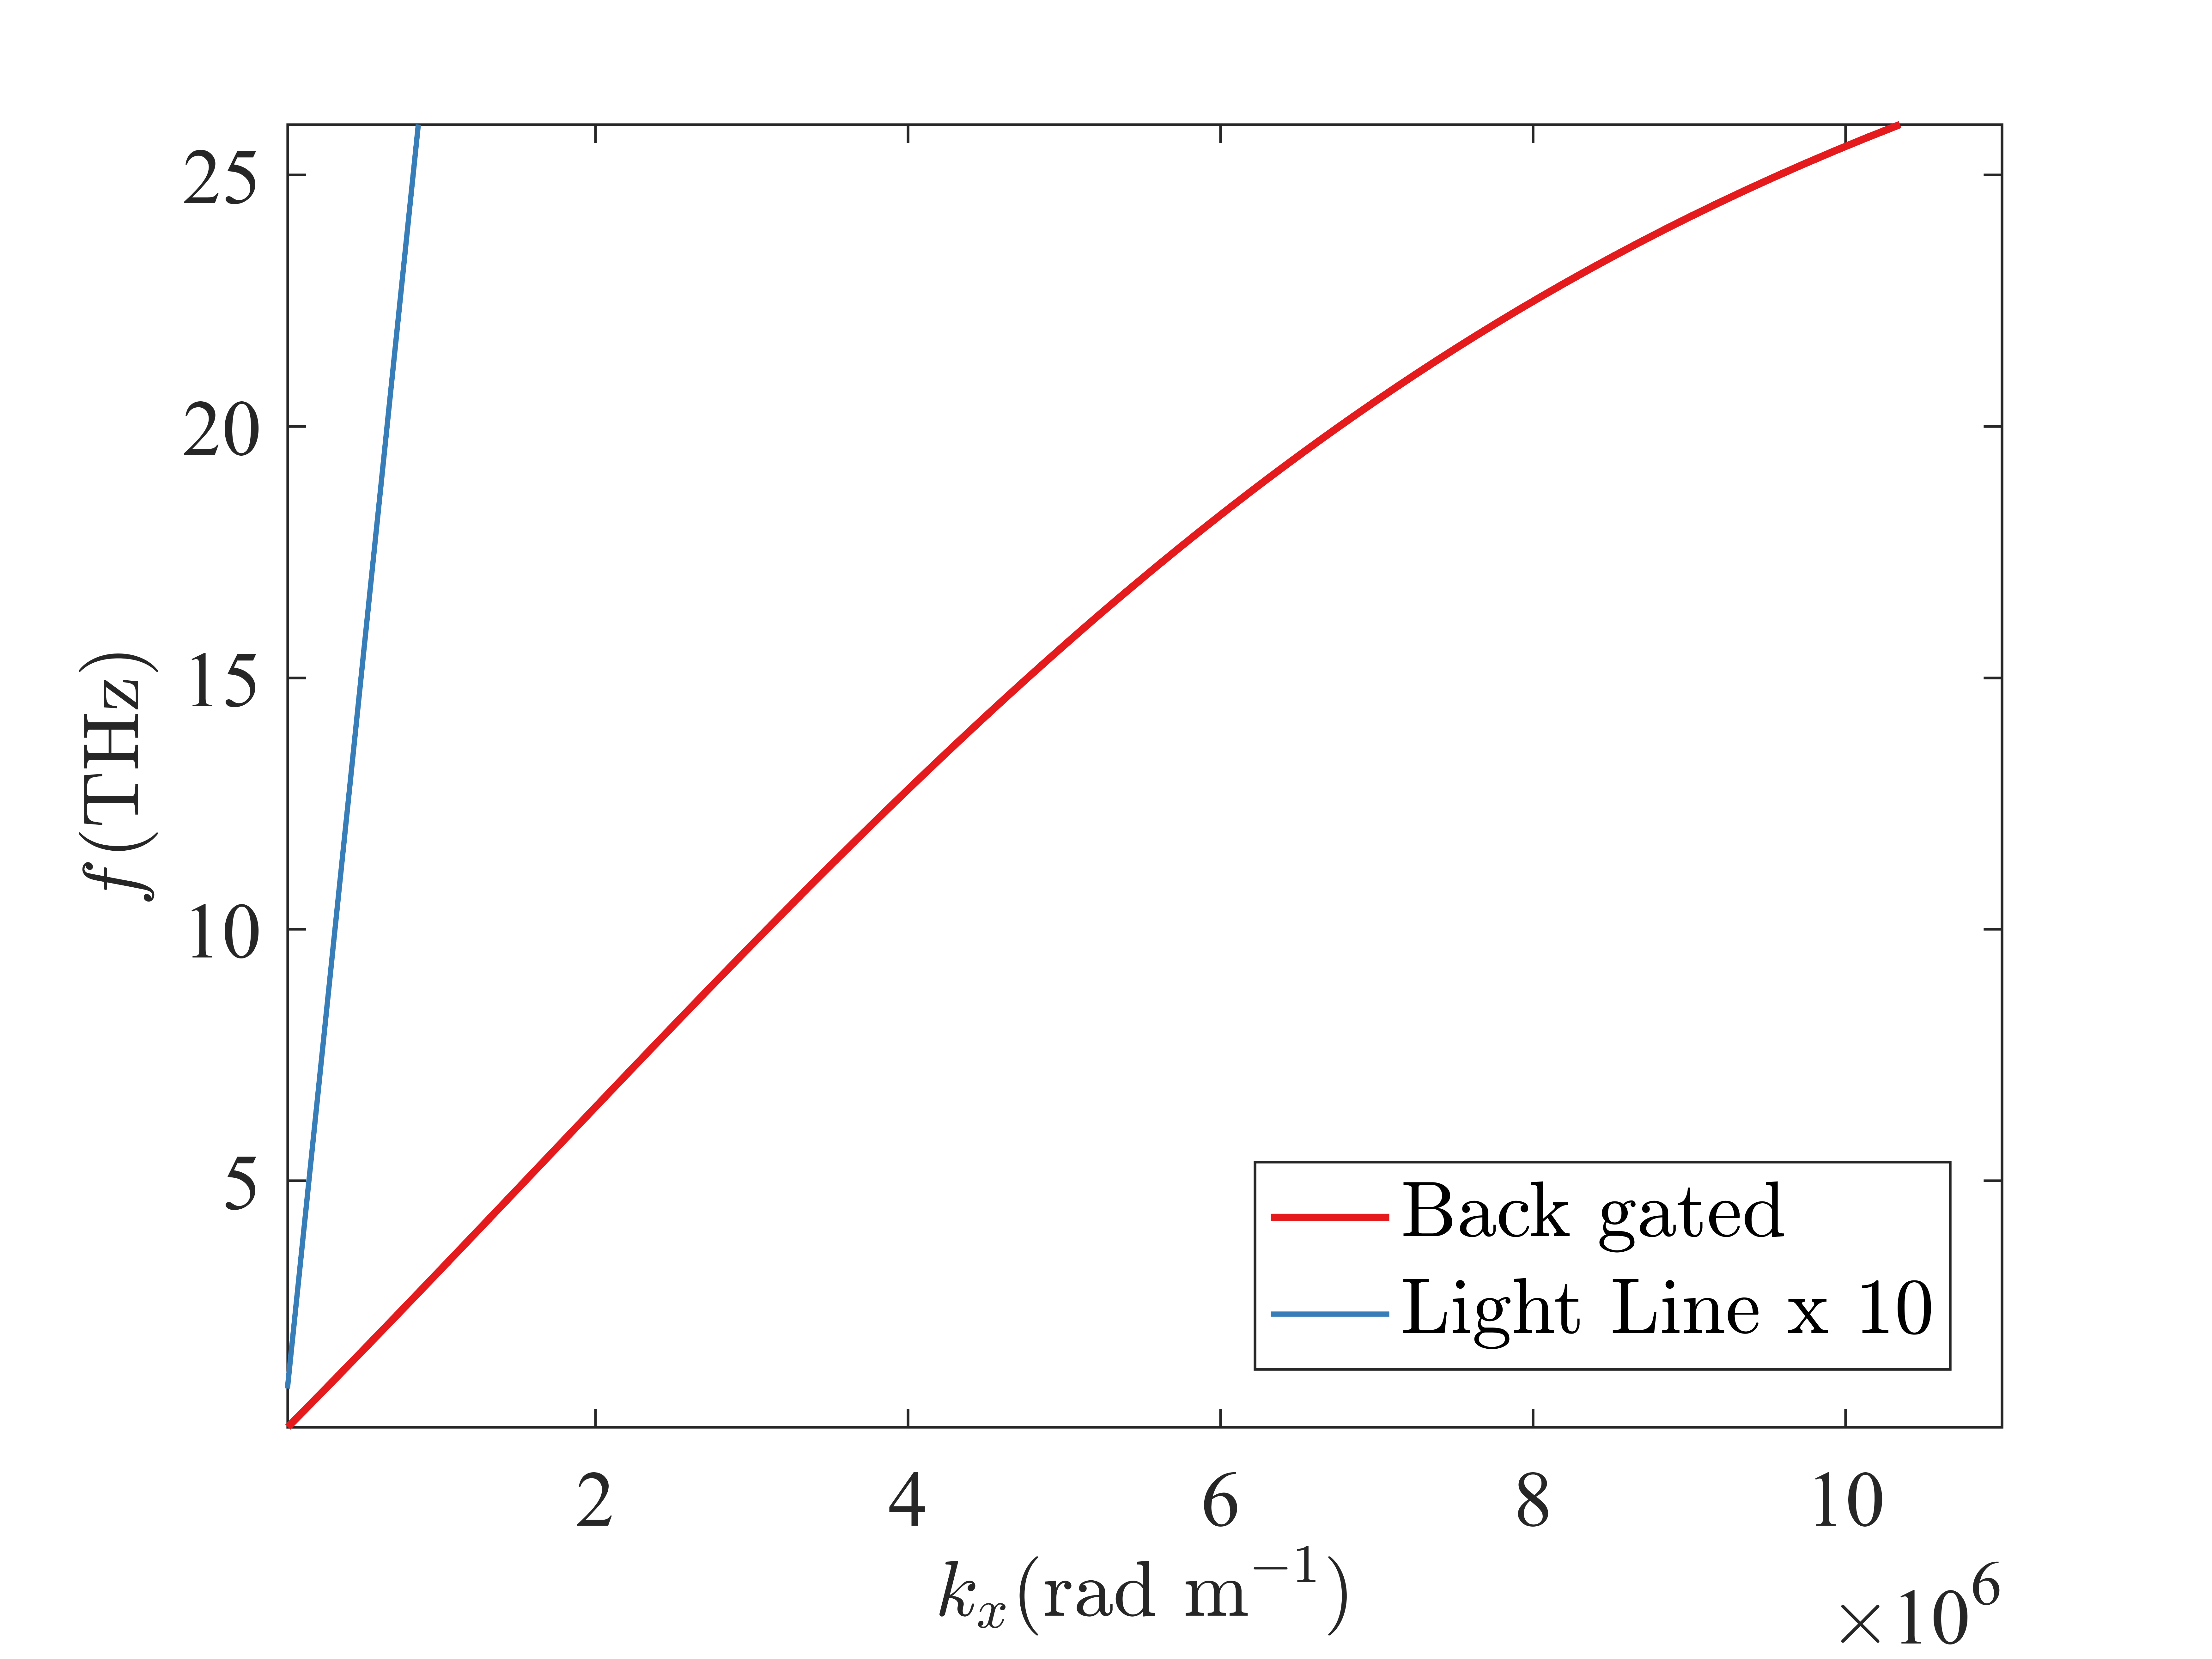
\includegraphics[height=2.2in]{gated_disp.tikz}
      \label{fig:dispersion}}
      \hfil
      \subfloat[]{\includegraphics[height=2.2in]{change_in_freq.tikz}
          \label{fig:tuning}}
  \caption{Dispersion relation of 2DEG embedded in region 2 of the heterostructure. Solid line: real part, dashed line: imaginary part}
  \label{fig:simulation1}
\end{figure}
%
%% Now discuss tunability of the 2DEG
Through the gate voltage $V_g$, the electron density $N_s$ of the channel can be varied using the relation:
%
\begin{equation}
  N_s = N_0 \times(1 - \frac{V_g}{V_T})
  \label{eq:tunability}
\end{equation}
%
where $N_0$ is the zero-bias density and $V_T$ is the gate threshold voltage of the transistor. For a channel terminated by highly conducting source and drain terminals at each side, the plasma frequency as a function of carrier density is expressed as \cite{Popov2008}:
%
\begin{equation}
  \O_p = \sqrt{\frac{N_s \e^2 d}{m_{\ast} \E}} \frac{\pi}{L}
  \label{eq:plasma_frq}
\end{equation}
%
where $\E$ is the average permittivity of the surrounding media. Using \eqref{eq:tunability} and \eqref{eq:plasma_frq}, the tunability of plasma waves assuming a gate threshold voltage of $-0.764 \mathrm{V}$ is shown in Fig. \ref{fig:tuning}. Normalized standing wave patterns tuned to different frequencies are shown in Fig. \ref{fig:s_waves} that were simulated using commercial full-wave electromagnetic software \cite{comsol}.
%
\begin{figure}[t!]
  \subfloat[]{\includegraphics[height=2.2in]{figures/shifted.tikz}
      \label{fig:shift}}
      \hfil
  \subfloat[]{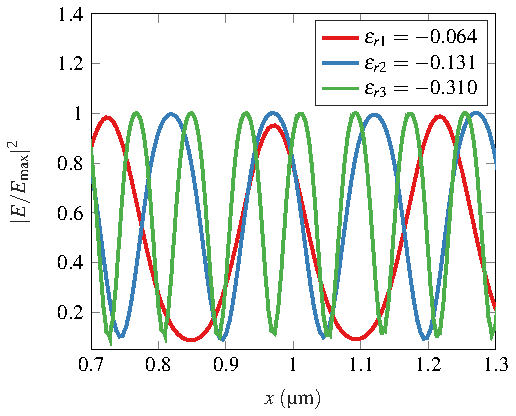
\includegraphics[height=2.2in]{tuning.tikz}
  \label{fig:s_waves}}
  \caption{Dispersion relation of 2DEG embedded in region 2 of the heterostructure. Solid line: real part, dashed line: imaginary part}
  \label{fig:simulation1}
\end{figure}
%
\subsection{Image Reconstruction}
%
Consider $I(\v r)$ as the sinusoidal illumination intensity:
%
\begin{equation}
  I(\v r) = 1 + \cos(\v k_{\p} \cdot \v r + \phi)
  \label{eq:intensity}
\end{equation}
where $\v k_{\p} = k_x \v{\^{x}} + k_y \v{\^{y}}$ is the spatial frequency wavevector,  $\v r = x \v{\^{x}} +  y \v{\^{y}}$ is the two-dimensional positional vector and $\phi$ is the pattern phase. The image of a sample $F(\v r)$ observed through a microscope can be expressed as:
%
\begin{equation}
  M(\v r) = \left[ F(\v r) \cdot I(\v r) \right] \otimes H(\v r)
  \label{eq:m_spatial_image}
\end{equation}
%
where $H(\v r)$ is the point spread function (PSF) of the microscope, and $\cdot, \otimes$ denote multiplication and convolution operations in the spatial domain respectively. A frequency domain representation of the image obtained by taking the Fourier transform of \eqref{eq:m_spatial_image} is expressed as:
%
\begin{equation}
  \begin{split}
    \ti M(\v k) &= \left[ \ti F(\v k) \otimes \ti I(\v k) \right] \cdot \ti H(\v k) \\
     &= \frac{1}{2} \left[ 2\ti F(\v k) + \ti F(\v k - \v k_{\p}) \e^{- \j \phi} + \ti F(\v k + \v k_{\p}) \e^{\j \phi} \right] \cdot \ti H(\v k)
  \end{split}
  \label{eq:m_ft}
\end{equation}

where $\sim$ over the letters indicates a frequency domain term and $\ti H(k)$ is the optical transfer function (OTF) of the microscope. A spatial frequency representation of the scheme is illustrated in Fig. \ref{fig:sim}. Assuming a numerical aperture of (NA) of unity, the OTF can be described by a circular disc as shown in Fig. \ref{fig:sim}(a) where the passband is bounded by $\sqrt{k_x^2 + k_y^2} = \nu$. As evident in \eqref{eq:m_ft}, a sinusoidal illumination pattern has three frequency components which generates an image that is a linear combination of the sample along with two shifted versions as shown in Fig. \ref{fig:sim}(b). To reconstruct the sample, three different images need to be captured with each possessing a different phase term $\phi$. The process can be expressed as a system of linear equations,
%
\begin{equation}
  \ti H(\v k) \cdot
  \begin{bmatrix}
    \ti F(\v k) \\
    \ti F(\v k - \v k_{\p}) \\
    \ti F(\v k + \v k_{\p})
  \end{bmatrix}
  =
  \begin{bmatrix}
    2 & \e^{-\j \phi_1} & \e^{\j \phi_1} \\
    2 & \e^{-\j \phi_2} & \e^{\j \phi_2} \\
    2 & \e^{-\j \phi_3} & \e^{\j \phi_3} \\
  \end{bmatrix}^{-1}
  \begin{bmatrix}
   \ti M_1(\v k) \\
   \ti M_2(\v k) \\
   \ti M_3(\v k)
  \end{bmatrix}
  \label{eq:reconstruction_algo}
\end{equation}
%
\begin{figure}[t!]
  \centering
  \def\svgwidth{.75\linewidth}
  \input{figures/psim.pdf_tex}
  \caption{Resolution enhancement through SIM: (a) Diffraction limited observable region in frequency domain.  Moiré effect using a sinusoidal illumination pattern bringing high frequency content under the observable region. Sample illuminated at different plasma frequencies: (b)-(d). (e) Effective resolution enhancement of $k_{\p 1 + \upsilon}$ in two dimensions obtained after rotating the sample w}
  \label{fig:sim}
\end{figure}
%
The phase shifts in \eqref{eq:reconstruction_algo} are known beforehand. Frequency content of the sample up to $k_{\p}$ can, therefore be observed due the Moiré effect which transports the high frequency information in to the observation region. To achieve two-dimensional enhancement in resolution, either the sample must be rotated about the optical axis of the microscope or the angular distribution of the illumination needs to be varied. The performance in terms of imaging speed can be improved by exciting the sample further with a pulse having energy higher than the plasmon illumination \cite{Zeng2015}. In the spatial frequency space, this corresponds to an enlarged observable region depicted by lighter colored discs in Fig. \ref{fig:sim}. This way fewer plasmon frequencies are needed to cover the complete range of frequencies.
%
In this work, an external plane wave is used to shift the plasma wave pattern laterally in the sample stage. The electric field of a TM polarized plane wave is expressed as, $\v E_{ext} = a \v{\^x} + b \v{\^z}$. The total field at the surface is the sum of the plasmonic field and external plane wave. The total intensity is then expressed as:
%
\begin{equation}
  \begin{split}
    \vert E \vert^2 &= (a + \cos k_{\p}x)^2 + (b + \sin k_{\p}x)^2 \\
    &=  a^2 + b^2 + 1 + 2 \chi \cos(k_{\p}x + \psi)
  \end{split}
  \label{eq:shift}
\end{equation}
%
where $k_{\p}$ is the spatial frequency of plasma wave, $\chi = \sqrt{a^2 + b^2}$ and $\psi = \atan (b/a)$. The field components $a$ and $b$ are controlled by changing the incident angle of the plane wave. Using a commercial full-wave electromagnetic simulation tool \cite{comsol}, the pattern shifting is shown in An example of phased shift is shown in Fig. \ref{fig:shift}.

%%%%%%%%%%%%%%%
%%%%%%%%%%%%%%%
%%%%%%%%%%%%%%%
%%%%%%%%%%%%%%%
%%%%%%%%%%%%%%%
%%%%%%%%%%%%%%%
%%%%%%%%%%%%%%%
%%%%%%%%%%%%%%%
%%%%%%%%%%%%%%%
\section{Simulated Results}
%
We consider a sample with atom distribution shown in Fig. \ref []. Each particle has a diameter of $1$ nm. First, the distribution is transformed in the spatial frequency domain by taking the Fourier transform. In the second step, the image is reconstructed via the inverse Fourier transform where only frequencies up to $k_{\p}$ are considered. To demonstrate the tunability of the Simulations were computed with plasmon wavenumbers taken $39.5 k_0$ and $80 k_0$ at $25~\mathrm{THz}$ and the results are shown in Fig. \ref{} with respective resolution of $79~\mathrm{nm}$ and $39.5~\mathrm{nm}$. In the first case, particles that are separated with a distance less than the resolution can not be resolved and appear as a contiguous blurry streak in the reconstructed image. When the resolution is increased by
%
At cryogenic temperatures, the plasmons exhibit near loss-less behavior in the 2DEG where the real part of the wavenumber is at least three orders of magnitude greater than the imaginary part. However, as the temperature rises, the reduced electron mobility resulting due to electron scattering introduces a plasma wave decay factor such . To account for the loss, the plasma

% Discuss loss in the scheme
\begin{figure}[t!]
  \subfloat[]{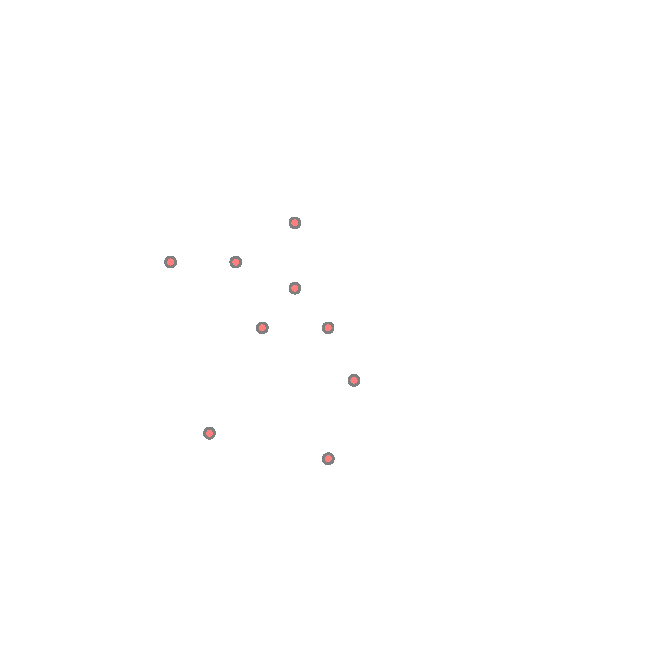
\includegraphics[height = 1.9in]{test_sample.tikz}
  \label{fig:test}} \hfil
  \subfloat[]{\includegraphics[height = 1.9in]{plsim_39.tikz}
  \label{fig:sim_lo}} \hfil
  \subfloat[]{\includegraphics[height = 1.9in]{plsim_80.tikz}
  \label{fig:sim_hi}}
  \caption{Dispersion relation of 2DEG embedded in region 2 of the heterostructure. Solid line: real part, dashed line: imaginary part}
  \label{fig:simulation}
\end{figure}
%%%%%%%%%%%%%%%
%%%%%%%%%%%%%%%
%%%%%%%%%%%%%%%
%%%%%%%%%%%%%%%
%%%%%%%%%%%%%%%
%%%%%%%%%%%%%%%
%%%%%%%%%%%%%%%
%%%%%%%%%%%%%%%
%%%%%%%%%%%%%%%
\section{Conclusion}
%

%%%%%%%%%%%%%%%
%%%%%%%%%%%%%%%
%%%%%%%%%%%%%%%
\clearpage % Force Bibliography to the end of document on a new page.
% \printbibliography
% \addbibresource{zubairy}
\bibliography{zubairy}
\bibliographystyle{ieeetran}

\end{document}
